% Asal-usul (tidak pernah dicetak): lihat sources/outline_sources.md (Tahun 1: pabrik karbonat; terumbu dan platform; ooze pelagis dan kedalaman kompensasi karbonat; ooze silika; urutan evaporit). Nilai soal latihan dan soal dalam kalkulator skrap Buku 3 calc/ch22.py; data gambar dari figdata/bachelor-1/evaporation.py dan ccd_flank.py. Kalsit, aragonit dan dolomit milik bab 7; hukum kedalaman--umur milik bab 13; salinitas milik Buku 1 (kelas 8); batu kapur milik Buku 1 (kelas 6, prosa); sistem karbonat dan alkalinitas milik buku-buku kimia dan biologi (diingat kembali, tidak pernah didefinisikan). Penurunan pulau vulkanik di bawah terumbu milik volume Tahun ke-2 (pulau samudra); diagenesis (dolomitisasi, rijang, gipsum menjadi anhidrit) milik bab 23; upwelling milik bab 29.
\chapter{Sedimen karbonat, silika dan evaporit}\label{ch:b1:chemical-biogenic-sediments}

Tebing-tebing kapur putih yang saling berhadapan di seberang laut sempit antara Inggris dan Prancis tampak seperti batuan yang paling biasa. Di bawah mikroskop elektron mereka ternyata tersusun dari lempengan-lempengan kalsit yang sangat kecil tak terhitung jumlahnya, yang ditinggalkan oleh alga bersel tunggal yang mengapung di laut yang menutupi kawasan itu. Sebuah \omterm{def:b1:chemical-biogenic-sediments:reef}{terumbu} yang dilihat dari perahu adalah kisah yang sama di ujung skala lain: batu kapur yang sedang terbentuk, dibangun oleh karang dan alga yang mengambil kalsium dan karbonat dari air dan mengubahnya menjadi batu. Tidak semua sedimen diangkut; banyak yang dibuat di tempat ia berada, oleh makhluk hidup atau oleh air itu sendiri ketika menguap. Bab ini mengikuti tiga keluarga besar sedimen ini --- karbonat, \omterm{def:b1:chemical-biogenic-sediments:ooze}{ooze silika} dan \omterm{def:b1:chemical-biogenic-sediments:evaporite}{evaporit} --- dari kimia laut yang memasoknya hingga batuan yang mereka tinggalkan.

\begin{recall}
Batu kapur adalah batuan sedimen yang tersusun dari kalsit, sering dari cangkang, dan ia berbusa dalam asam encer (Buku~1, kelas~6). Kalsit dan aragonit adalah dua \omterm{def:b1:rock-forming-minerals:polymorph}{polimorf} \ce{CaCO3}, dengan massa jenis \qty{2.71}{g.cm^{-3}} dan \qty{2.93}{g.cm^{-3}}, dan dolomit \ce{CaMg(CO3)2}, dengan massa jenis \qty{2.84}{g.cm^{-3}}, adalah karbonat kalsium dan magnesium (\cref{ch:b1:rock-forming-minerals}). Salinitas air laut adalah massa garam yang larut dalam satu kilogram airnya (Buku~1, kelas~8). Dalam air, karbon dioksida, ion hidrogen karbonat dan ion karbonat dihubungkan oleh kesetimbangan asam--basa, dan alkalinitas mengukur basa yang mampu menyerap ion hidrogen (buku-buku kimia); sistem karbonat laut ikut serta dalam siklus karbon (buku-buku biologi). Dasar laut mendalam seiring umur sebagai $d = d_r + C\sqrt t$ (\cref{thm:b1:rifts-ridges-margins:depth-age}).
\end{recall}
% ledger: webmineral:polymorphs, hom:calcite, webmineral:others

\section{Pabrik karbonat}\label{sec:b1:chemical-biogenic-sediments:factory}

Air laut mengandung kalsium dan karbon anorganik terlarut, sebagian besar sebagai ion hidrogen karbonat. Kalsium karbonat terbentuk dari keduanya melalui reaksi
\[
\ce{Ca^2+ + 2 HCO3- -> CaCO3 + CO2 + H2O}, \qquad
\ce{Ca^2+ + CO3^2- -> CaCO3},
\]
yang pertama melepaskan satu molekul karbon dioksida untuk setiap satu karbonat yang diendapkan. Air permukaan tropis yang hangat jenuh lewat batas terhadap kalsium karbonat, tetapi jarang mengendap sendiri: hampir semua dibuat oleh makhluk hidup, yang membayar energi untuk membangun cangkang dan kerangka mereka dan mengendalikan \omterm{def:b1:rock-forming-minerals:mineral}{mineral} yang mereka gunakan. Karang dan alga hijau membangun aragonit; alga merah dan banyak foraminifera membangun kalsit, sebagian kaya magnesium; moluska menggunakan salah satu atau keduanya.

\begin{definition}[Pabrik karbonat]\label{def:b1:chemical-biogenic-sediments:factory}
\emph{Pabrik karbonat}\index{pabrik karbonat} suatu laut adalah himpunan organisme dan proses yang menghasilkan sedimen kalsium karbonat di tempat ia ditemukan, bukan membawanya dari tempat lain. Produknya adalah butiran kerangka (cangkang dan kerangka utuh atau pecah), lumpur karbonat, butiran berselubung dan kerangka kaku \omterm{def:b1:chemical-biogenic-sediments:reef}{terumbu}.
\end{definition}

Pabrik paling kaya bekerja di air yang hangat, jernih, dangkal dan bermandikan cahaya, jauh dari lumpur sungai, yang akan mengubur produsennya dan mengaburkan cahaya yang dibutuhkan alga. Sedimennya dibuat oleh dasar laut itu sendiri: puing karang dan alga, cangkang moluska dan foraminifera bersel tunggal yang hidup di dasar, serta jarum aragonit yang dilepaskan oleh alga hijau, yang mengendap sebagai lumpur kapur. Di tempat air bergolak dan jenuh lewat batas, butiran yang digulingkan oleh ombak dan pasang surut menumbuhkan selubung karbonat, lapis demi lapis, di sekeliling inti, butir pasir atau pecahan cangkang, menjadi \omterm{def:b1:chemical-biogenic-sediments:reef}{ooid} bulat (\cref{def:b1:chemical-biogenic-sediments:reef}). Pabrik kedua bekerja di samudra terbuka, jauh dari pantai mana pun: plankton yang hidup di lapisan permukaan yang bermandikan cahaya membangun cangkang dan lempengan kalsit yang kecil, yang berjatuhan ke dasar laut dalam (\cref{sec:b1:chemical-biogenic-sediments:oozes}).
% ledger: og:carbonates

Seberapa cepat sebuah pabrik membangun diukur dengan anggaran karbonatnya, massa karbonat yang dihasilkan dan dipertahankan di tempatnya setiap tahun pada satu meter persegi, setelah kehilangan akibat organisme pengebor, pemakan rumput laut dan ombak. Ia diubah menjadi laju pertumbuhan vertikal dengan neraca massa.

\begin{proposition}[Akresi dari anggaran karbonat]\label{prop:b1:chemical-biogenic-sediments:accretion}
Misalkan suatu dasar laut mempertahankan massa bersih $G$ kalsium karbonat per satuan luas dan per satuan waktu, sebagai endapan yang butiran padatnya memiliki massa jenis $\rho_s$ dan yang porositasnya, yakni fraksi volumenya yang diambil oleh pori-pori, adalah $\phi$. Maka dasar itu naik dengan laju
\[
a = \frac{G}{\rho_s\,(1-\phi)}.
\]
\end{proposition}

\begin{proof}
Dalam waktu $\mathrm dt$ satu satuan luas menerima massa $G\,\mathrm dt$ karbonat padat, yang mengisi volume $G\,\mathrm dt/\rho_s$ butiran. Butiran ini membentuk fraksi $1-\phi$ dari lapisan baru, yang tebalnya karena itu $G\,\mathrm dt/(\rho_s(1-\phi))$. Membagi dengan $\mathrm dt$ memberikan $a$.
\end{proof}

Hasil kali $\rho_s(1-\phi)$ adalah massa jenis curah kering endapan. Di \omterm{def:b1:chemical-biogenic-sediments:reef}{terumbu} Kepulauan Chagos di Samudra Hindia, 28 \omterm{def:b1:chemical-biogenic-sediments:reef}{terumbu} yang diukur pada 2015 memiliki anggaran rerata \qty{3.7}{kg} \ce{CaCO3} per meter persegi dan per tahun, dan yang didominasi karang \emph{Acropora} bercabang \qty{8.4}{kg}, tumbuh sekitar \qty{4.2}{mm} setahun; dengan proposisi, kedua angka ini bersama-sama berarti massa jenis curah kering \qty{2000}{kg.m^{-3}}, yakni kerangka \omterm{def:b1:chemical-biogenic-sediments:reef}{terumbu} dengan sekitar sepertiga ruang pori (\cref{exo:b1:chemical-biogenic-sediments:3}). \omterm{def:b1:chemical-biogenic-sediments:reef}{Terumbu} yang sama telah kehilangan lebih dari sembilan persepuluh karangnya dalam peristiwa pemanasan 1998, dan anggaran mereka menunjukkan seberapa cepat sebuah \omterm{def:b1:chemical-biogenic-sediments:reef}{terumbu} dapat membangun kembali.
% ledger: perry:chagos

\section{Terumbu dan platform}\label{sec:b1:chemical-biogenic-sediments:reefs}

Di tempat pabrik membangun kerangka kaku, ia dapat berdiri dari dasar laut melawan ombak.

\begin{definition}[Terumbu, platform karbonat, ooid]\label{def:b1:chemical-biogenic-sediments:reef}
Sebuah \emph{terumbu}\index{terumbu} adalah tumpukan karbonat yang kerangka organismenya (karang, alga atau lainnya, yang tumbuh di tempatnya dan saling mengikat serta menyemen) berdiri di atas dasar laut sekitarnya dan menahan ombak. Sebuah \emph{platform karbonat}\index{platform karbonat} adalah tubuh tebal karbonat air dangkal yang puncaknya datar mendekati permukaan laut dan dibatasi oleh lereng yang turun ke air yang lebih dalam. Sebuah \emph{ooid}\index{ooid} adalah butiran bulat berukuran pasir yang tersusun dari lapisan-lapisan konsentris kalsium karbonat yang tumbuh di sekeliling inti ketika ia bergulir di air yang bergolak; batuan yang tersusun dari ooid disebut oolit.
\end{definition}
% ledger: og:carbonates

\omterm{def:b1:chemical-biogenic-sediments:reef}{Terumbu} karang modern hadir dalam tiga jenis, dinamai oleh para pelaut yang memetakannya jauh sebelum ada yang mengebor menembusnya. Sebuah \omterm{def:b1:chemical-biogenic-sediments:reef}{terumbu} \emph{tepi} menempel pada pantai pulau atau benua. Sebuah \omterm{def:b1:chemical-biogenic-sediments:reef}{terumbu} \emph{penghalang} dipisahkan dari daratan oleh laguna, yang dapat lebar dan berkedalaman puluhan meter: penghalang di timur laut Australia membentang, dengan celah-celah, hampir seribu mil, mengurung laut sedalam 10 hingga 25 depa, sekitar 18 hingga \qty{46}{m}. Sebuah \emph{atol} adalah cincin \omterm{def:b1:chemical-biogenic-sediments:reef}{terumbu}, yang menopang pulau-pulau rendah dari pasir karang, mengelilingi laguna tanpa daratan sama sekali di dalamnya.

\begin{omfigure}
\begin{tikzpicture}[font=\footnotesize, scale=0.72]
% three reef types in cross-section (schematic): a volcanic cone y = 2 - s - 0.75|x - 4|
% subsided by s (0, 0.8, 1.6), sea level at y = 1; the reef grows up from its first
% position, the foot of the fringing reef at (2, 0.5) moving down with the cone
\foreach \s/\yo/\lab/\name in {0/0/a/terumbu tepi, 0.8/-3.8/b/terumbu penghalang, 1.6/-7.6/c/atol} {
  \begin{scope}[yshift=\yo cm]
    \begin{scope}
      \clip (0,-1.3) rectangle (8,2.3);
      \fill[omSea] (0,-1.3) rectangle (8,1.0);
      \draw[lith basalt] (-1,2-\s-3.75) -- (4,2-\s) -- (9,2-\s-3.75) -- cycle;
    \end{scope}
    \draw[omSea!60!black] (0,1.0) -- (8,1.0);
    \node[anchor=west, font=\scriptsize] at (8.05,1.0) {permukaan laut};
    \node[anchor=west] at (0,2.05) {(\lab) \name};
    \draw[black!70] (1.6,1.55) node[anchor=east, font=\scriptsize] {terumbu} -- (2.2,1.02);
  \end{scope}
}
% (a) fringing reef: wedges against the shore
\fill[lith reef limestone, draw=black!70] (2.0,0.5) -- (2.15,1.0) -- (2.667,1.0) -- cycle;
\fill[lith reef limestone, draw=black!70] (6.0,0.5) -- (5.85,1.0) -- (5.333,1.0) -- cycle;
\node[anchor=west, font=\scriptsize] at (4.9,1.75) {pulau vulkanik};
% (b) barrier reef: the cone has sunk by 0.8, the reef has grown up, a lagoon opens
\begin{scope}[yshift=-3.8cm]
  \fill[lith reef limestone, draw=black!70] (2.0,-0.3) -- (2.15,1.0) -- (2.6,1.0) -- (2.55,0.1125) -- cycle;
  \fill[lith reef limestone, draw=black!70] (6.0,-0.3) -- (5.85,1.0) -- (5.4,1.0) -- (5.45,0.1125) -- cycle;
  \draw[black!70] (3.2,0.85) -- (3.45,1.55) node[anchor=south west, font=\scriptsize, inner sep=1pt] {laguna};
\end{scope}
% (c) atoll: the cone has sunk by 1.6 and is drowned; the reef ring encloses a lagoon
\begin{scope}[yshift=-7.6cm]
  \fill[lith limestone, draw=black!50] (2.55,-0.6875) -- (2.55,0.55) -- (5.45,0.55) -- (5.45,-0.6875) -- (4,0.4) -- cycle;
  \fill[lith reef limestone, draw=black!70] (2.0,-1.1) -- (2.15,1.0) -- (2.6,1.0) -- (2.55,-0.6875) -- cycle;
  \fill[lith reef limestone, draw=black!70] (6.0,-1.1) -- (5.85,1.0) -- (5.4,1.0) -- (5.45,-0.6875) -- cycle;
  \node[font=\scriptsize] at (4,0.78) {laguna};
  \node[font=\scriptsize, fill=omLithLime, inner sep=1pt] at (4,0.05) {sedimen laguna};
\end{scope}
% photograph
\node[anchor=north west, inner sep=0] at (10.75,2.3) {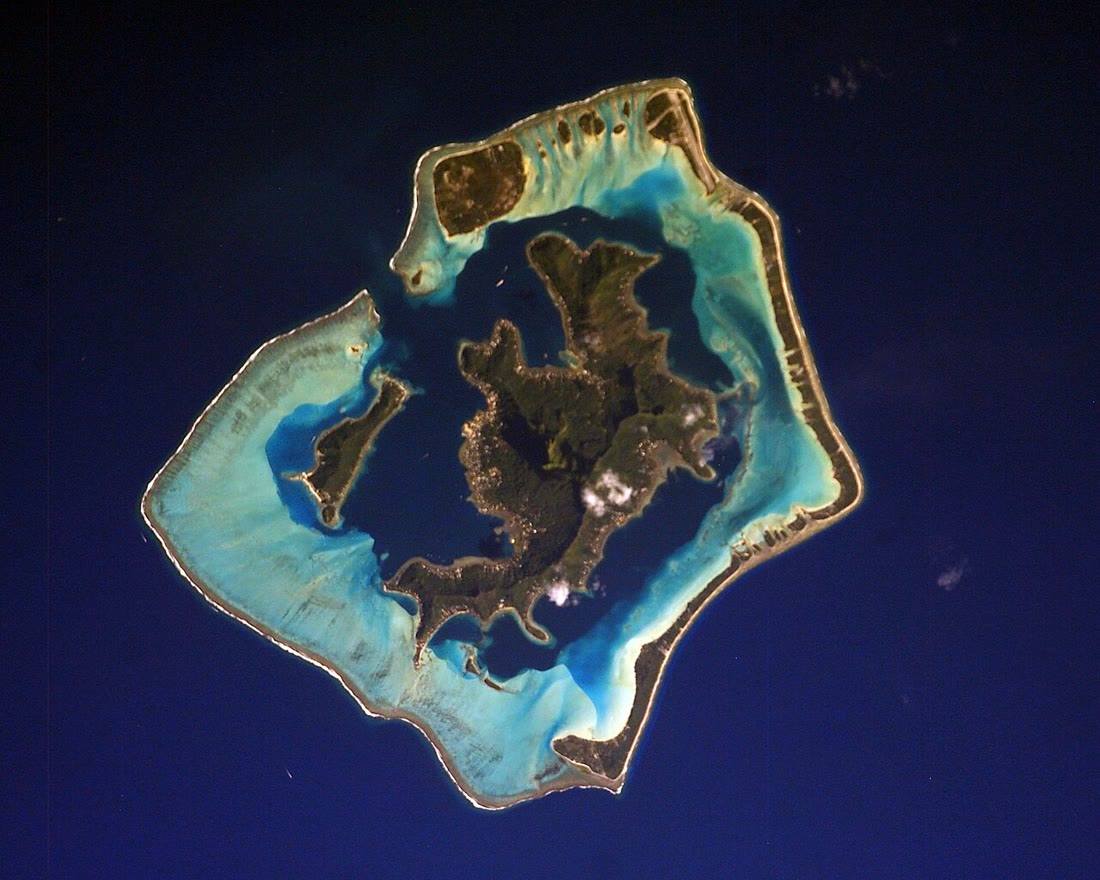
\includegraphics[height=6.9cm]{images/book3/b1-bora-bora.jpg}};
\end{tikzpicture}

{\small Kiri: tiga jenis \omterm{def:b1:chemical-biogenic-sediments:reef}{terumbu} karang dalam penampang (skematis, skala vertikal sangat dilebih-lebihkan), digambar seperti yang dijelaskan Darwin: (a)~\omterm{def:b1:chemical-biogenic-sediments:reef}{terumbu} yang mengelilingi pulau vulkanik; (b)~pulau telah tenggelam dan \omterm{def:b1:chemical-biogenic-sediments:reef}{terumbu}, yang tumbuh ke atas, telah menjadi \omterm{def:b1:chemical-biogenic-sediments:reef}{terumbu} penghalang yang dipisahkan dari pantai oleh laguna; (c)~pulau telah tenggelam dari pandangan dan \omterm{def:b1:chemical-biogenic-sediments:reef}{terumbu} menjadi atol di sekeliling laguna yang berdasar sedimen karbonat. Kanan: Bora Bora, pulau vulkanik di dalam laguna yang dikelilingi \omterm{def:b1:chemical-biogenic-sediments:reef}{terumbu} penghalang dengan pulau-pulau rendah di atasnya, difoto oleh seorang astronot dari Stasiun Luar Angkasa Internasional pada 19 Maret 2003 (NASA, domain publik, melalui Wikimedia Commons).}
\label{fig:b1:chemical-biogenic-sediments:reefs}
\end{omfigure}
% ledger: darwin:reefs, commons:bora-bora

\begin{history}[Terumbu di atas fondasi yang tenggelam, 1837--1842]
Dalam pelayaran \emph{Beagle}, Charles Darwin berlayar di antara \omterm{def:b1:chemical-biogenic-sediments:reef}{terumbu} Samudra Pasifik dan Hindia. Ia bernalar dari satu fakta: karang pembangun \omterm{def:b1:chemical-biogenic-sediments:reef}{terumbu}, simpulnya, pada umumnya tidak berkembang lebih dalam daripada antara 20 dan 30 depa, sekitar 37 hingga \qty{55}{m}. Namun \omterm{def:b1:chemical-biogenic-sediments:reef}{terumbu} penghalang dan atol naik dari air dalam, jauh di bawah batas itu. Fondasinya, ia berargumen, pastilah tenggelam, cukup lambat agar karang dapat menjaga puncaknya tetap di permukaan dengan tumbuh ke atas: \omterm{def:b1:chemical-biogenic-sediments:reef}{terumbu} yang mengelilingi pulau vulkanik menjadi \omterm{def:b1:chemical-biogenic-sediments:reef}{terumbu} penghalang ketika pulau itu tenggelam di dalamnya, dan menjadi atol ketika pulau itu telah lenyap. Ia membacakan teorinya di hadapan Masyarakat Geologi London pada 31 Mei 1837 dan menerbitkannya pada 1842 dalam \emph{Struktur dan Persebaran \omterm{def:b1:chemical-biogenic-sediments:reef}{Terumbu} Karang}, dengan peta semua \omterm{def:b1:chemical-biogenic-sediments:reef}{terumbu} dunia yang diurutkan menjadi tiga jenis. Mengapa pulau samudra tenggelam, dan seberapa jauh, adalah soal pendinginan lempeng di bawahnya, yang dibahas dalam volume Tahun ke-2.
\end{history}
% ledger: darwin:reefs

\omterm{def:b1:chemical-biogenic-sediments:reef}{Terumbu} hanya bertahan jika puncaknya tetap berada di air dangkal tempat pembangunnya hidup. Permukaan laut berubah, dan fondasinya dapat turun; yang penting adalah jumlah keduanya, kenaikan relatif permukaan laut.

\begin{proposition}[Mengimbangi atau tenggelam]\label{prop:b1:chemical-biogenic-sediments:keep-up}
Misalkan puncak \omterm{def:b1:chemical-biogenic-sediments:reef}{terumbu} berada pada kedalaman $D_0$ di bawah permukaan laut dan tumbuh ke atas dengan laju $a$, sementara permukaan laut relatif naik dengan laju $r$, keduanya konstan. Maka kedalaman air di atas \omterm{def:b1:chemical-biogenic-sediments:reef}{terumbu} setelah waktu $t$ adalah
\[
D(t) = D_0 + (r - a)\,t .
\]
Jika $a \ge r$, \omterm{def:b1:chemical-biogenic-sediments:reef}{terumbu} mengimbangi laut (ketika $a > r$ puncaknya mencapai permukaan, dan sejak itu ia hanya dapat tumbuh ke samping); jika $a < r$ ia tertinggal, dan jika pembangunnya tidak dapat hidup lebih dalam dari $D_{\max}$, ia tenggelam setelah waktu $(D_{\max} - D_0)/(r - a)$.
\end{proposition}

\begin{proof}
Ukur tinggi ke atas dari suatu tanda tetap pada fondasi. Puncak \omterm{def:b1:chemical-biogenic-sediments:reef}{terumbu} berada di $h_0 + a t$ dan permukaan laut di $s_0 + r t$, sehingga kedalaman air di atas
puncak adalah $D = (s_0 - h_0) + (r - a)t = D_0 + (r-a)t$. Ketika $a > r$, $D$ mencapai nol pada $t = D_0/(a-r)$ dan \omterm{def:b1:chemical-biogenic-sediments:reef}{terumbu} tidak dapat tumbuh di atas laut. Ketika
$a < r$, $D$ tumbuh secara linier dan mencapai $D_{\max}$ ketika $(r-a)t = D_{\max} -
D_0$.
\end{proof}

\omterm{def:b1:chemical-biogenic-sediments:reef}{Terumbu} yang puncaknya telah tenggelam belum langsung mati, tetapi cahaya meredup, pembangunnya berganti dan pabrik melambat, sehingga \omterm{def:b1:chemical-biogenic-sediments:reef}{terumbu} yang mulai tertinggal makin tertinggal: \omterm{def:b1:chemical-biogenic-sediments:reef}{terumbu} dan platform yang tenggelam, ditutupi oleh sedimen laut dalam, ditemukan di lereng banyak pulau samudra dan dalam catatan batuan.

Selama jutaan tahun pabrik membangun \omterm{def:b1:chemical-biogenic-sediments:reef}{platform karbonat}, tubuh-tubuh tebal karbonat air dangkal yang tumbuh ketika fondasinya turun. Dua bentuk berulang
(lihat gambar di bawah). Sebuah \emph{paparan berbingkai} memiliki puncak datar, terlindung di belakang tepi \omterm{def:b1:chemical-biogenic-sediments:reef}{terumbu} dan gosong \omterm{def:b1:chemical-biogenic-sediments:reef}{ooid} di tepinya, yang memecah ombak; di belakangnya terbentang laguna tenang berisi lumpur kapur, dan di depannya lereng curam tempat balok dan puing yang lepas dari tepi jatuh ke cekungan. Sebuah \emph{rampa} miring sangat landai dari pantai ke cekungan tanpa patahan: gosong \omterm{def:b1:chemical-biogenic-sediments:reef}{ooid} dan tanggul cangkang tempat ombak mengaduk dasar, lalu lapisan puing cangkang yang disapu oleh badai, lalu lumpur kapur di bawah jangkauan ombak. Paparan berbingkai tumbuh terutama ke atas dan ke samping dari tepinya, sebuah rampa dengan memindahkan sabuk sedimennya ke arah pantai atau ke arah laut ketika permukaan laut naik atau turun.

\begin{omfigure}
\begin{tikzpicture}[font=\footnotesize, >={Stealth[length=4pt]}]
% (a) rimmed shelf and (b) ramp, schematic cross-sections
\begin{scope}
  \fill[omSea] (0,0.2) rectangle (7.2,2.0);
  \fill[lith limestone, draw=black!60] (0,0) -- (0,1.55) -- (4.3,1.55) -- (4.5,1.75) -- (4.9,1.75) -- (5.1,1.5) -- (6.4,0.35) -- (7.2,0.3) -- (7.2,0) -- cycle;
  \fill[lith reef limestone, draw=black!70] (4.3,1.55) -- (4.5,1.75) -- (4.9,1.75) -- (5.1,1.5) -- (4.8,1.05) -- (4.3,1.05) -- cycle;
  \draw[omSea!60!black] (0,2.0) -- (7.2,2.0);
  \node at (2.1,1.78) {laguna: lumpur kapur};
  \node[anchor=south, align=center, font=\scriptsize] at (4.7,2.05) {tepi terumbu dan\\ gosong ooid};
  \node[anchor=west, font=\scriptsize] at (5.6,1.2) {lereng: puing};
  \node[font=\scriptsize] at (6.75,0.75) {cekungan};
  \node at (3.6,-0.35) {(a) paparan berbingkai};
\end{scope}
\begin{scope}[xshift=8.0cm]
  \fill[omSea] (0,0.2) rectangle (7.2,2.0);
  \fill[lith limestone, draw=black!60] (0,0) -- (0,1.85) -- (7.2,0.55) -- (7.2,0) -- cycle;
  \draw[omSea!60!black] (0,2.0) -- (7.2,2.0);
  \draw[densely dashed, black!50] (0,1.6) -- (7.2,1.6) node[pos=1, anchor=south east, font=\scriptsize, inner sep=1pt] {ombak cuaca cerah mencapai};
  \draw[densely dashed, black!50] (0,1.0) -- (7.2,1.0) node[pos=1, anchor=south east, font=\scriptsize, inner sep=1pt] {ombak badai mencapai};
  \node[anchor=south, font=\scriptsize] at (0.9,2.05) {gosong ooid};
  \node[anchor=south, font=\scriptsize] at (3.4,2.05) {tanggul cangkang badai};
  \node[anchor=south, font=\scriptsize] at (6.1,2.05) {lumpur kapur};
  \node at (3.6,-0.35) {(b) rampa};
\end{scope}
\end{tikzpicture}

{\small Dua bentuk \omterm{def:b1:chemical-biogenic-sediments:reef}{platform karbonat} (skematis, lereng sangat dilebih-lebihkan). (a)~Paparan berbingkai: tepi \omterm{def:b1:chemical-biogenic-sediments:reef}{terumbu} dan gosong \omterm{def:b1:chemical-biogenic-sediments:reef}{ooid} memecah ombak, laguna tenang berisi lumpur kapur terbentang di belakangnya, dan puing yang lepas dari tepi jatuh menuruni lereng ke cekungan. (b)~Rampa miring landai dari pantai ke cekungan, sedimennya dipilah oleh kedalaman yang dijangkau ombak.}
\label{fig:b1:chemical-biogenic-sediments:platforms}
\end{omfigure}

\section{Ooze pelagis dan kedalaman kompensasi karbonat}\label{sec:b1:chemical-biogenic-sediments:oozes}

Jauh dari daratan, dasar laut hampir tidak menerima apa-apa dari benua selain debu halus yang diterbangkan angin. Yang jatuh di atasnya adalah kerangka plankton yang hidup di air bermandikan cahaya beberapa kilometer di atas: lempengan kalsit kokolitoforid dan cangkang foraminifera, frustul opal diatom dan kerangka radiolaria (tergambar sedikit lebih jauh). Hujan panjang kokolit ke dasar laut adalah proses utama yang membuat kapur dan sebagian besar batu kapur dunia.
% ledger: nasa:coccoliths-b3, og:carbonates

\begin{definition}[Ooze kapur, ooze silika]\label{def:b1:chemical-biogenic-sediments:ooze}
Ooze adalah sedimen pelagis berbutir halus, yang diendapkan di samudra terbuka, sebagian besar tersusun dari kerangka plankton. Ia menjadi \emph{ooze kapur}\index{ooze kapur} ketika kerangkanya dari kalsium karbonat, terutama kokolit dan foraminifera, dan \emph{ooze silika}\index{ooze silika} ketika kerangkanya dari opal, yakni silika amorf terhidrasi, terutama diatom dan radiolaria.
\end{definition}
% ledger: og:carbonates

\omterm{def:b1:chemical-biogenic-sediments:ooze}{Ooze kapur} menutupi sekitar separuh dasar laut dunia, tetapi hanya di atas kedalaman tertentu: di bawah sekitar \qty{4500}{m} mereka menghilang. Cangkang tidak berhenti jatuh di sana; mereka larut. Laut dalam itu dingin dan tekanannya tinggi, dan kelarutan kalsit naik seiring kedalaman, terutama karena tekanan, sementara konsentrasi ion karbonat dalam air umumnya turun seiring kedalaman (kimia kesetimbangan ini diingat kembali dari buku-buku kimia). Di bawah kedalaman tertentu air laut dalam tidak jenuh terhadap kalsit, dan cangkang yang sampai ke dasar larut makin cepat semakin dalam letaknya.
% ledger: britannica:ccd, slotnick:ccd-definitions

\begin{omfigure}
\begin{tikzpicture}
\node[inner sep=0] (a) at (0,0) {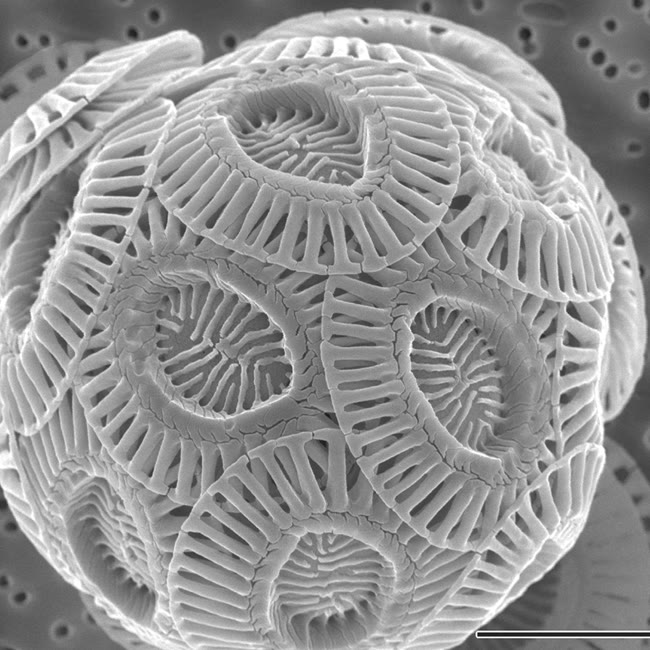
\includegraphics[height=4.3cm]{images/book3/b1-coccolithophore.jpg}};
\node[inner sep=0, anchor=west] (b) at ([xshift=0.25cm]a.east) {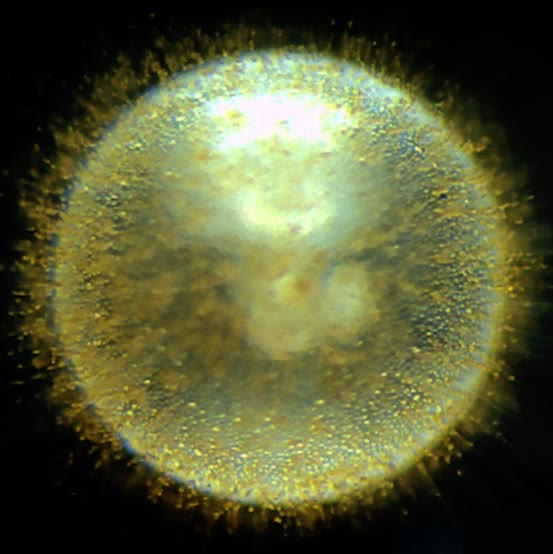
\includegraphics[height=4.3cm]{images/book3/b1-orbulina.jpg}};
\node[inner sep=0, anchor=west] (c) at ([xshift=0.25cm]b.east) {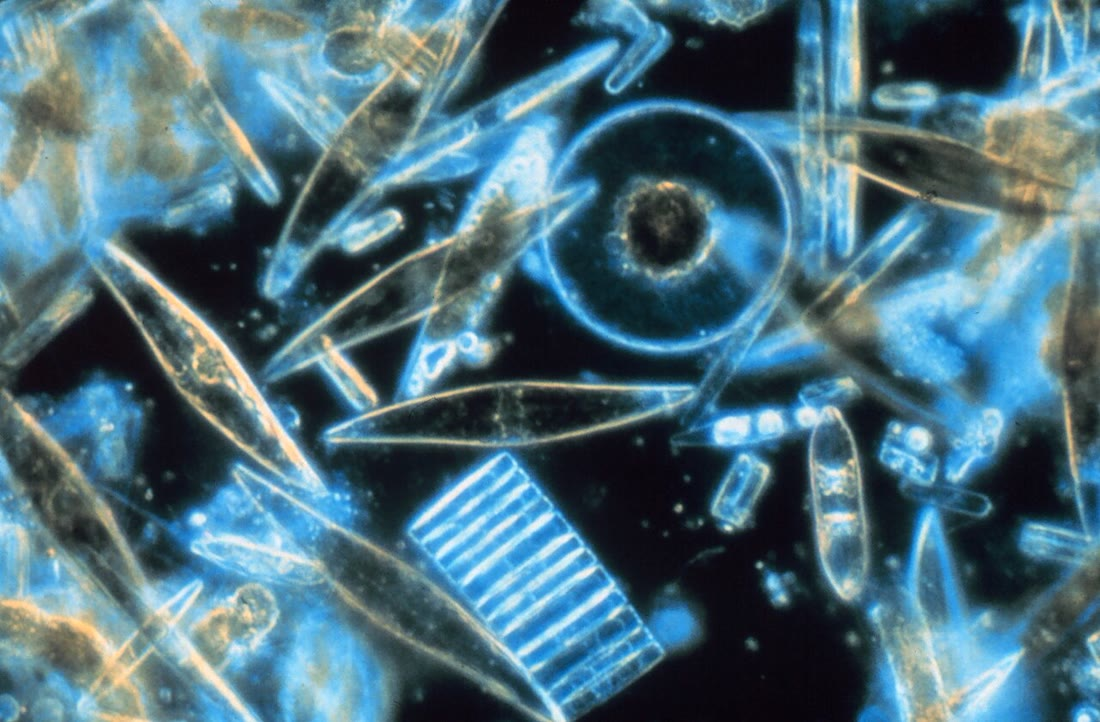
\includegraphics[height=4.3cm]{images/book3/b1-diatoms.jpg}};
\node[font=\footnotesize, anchor=north] at (a.south) {(a) sebuah kokolitoforid};
\node[font=\footnotesize, anchor=north] at (b.south) {(b) sebuah foraminifera};
\node[font=\footnotesize, anchor=north] at (c.south) {(c) diatom};
\end{tikzpicture}

{\small Pembuat ooze. (a)~Satu sel \emph{Emiliania huxleyi} yang berlapis kokolit, lempengan kalsitnya (mikroskop elektron pemindai; Alison R.~Taylor, Universitas Carolina Utara di Wilmington, CC~BY~2.5, melalui Wikimedia Commons). (b)~Foraminifera planktonik yang hidup, \emph{Orbulina universa}, dengan cangkang kalsitnya dikelilingi duri (mikroskop cahaya; H.~Takagi dan rekan penulis, 2019, CC~BY~4.0, melalui Wikimedia Commons). (c)~Diatom hidup dari es laut di Teluk McMurdo, Antartika, masing-masing dalam frustul opalnya (mikroskop cahaya; Gordon T.~Taylor, Universitas Stony Brook, NOAA, domain publik, melalui Wikimedia Commons).}
\label{fig:b1:chemical-biogenic-sediments:plankton}
\end{omfigure}
% ledger: commons:ehux, commons:orbulina, commons:diatoms-noaa

\begin{definition}[Lisoklin, kedalaman kompensasi karbonat]\label{def:b1:chemical-biogenic-sediments:ccd}
\emph{Lisoklin}\index{lisoklin} adalah kedalaman di laut di bawah mana pelarutan kalsit di dasar laut pertama kali tampak dalam sedimen dan lajunya naik tajam. \emph{Kedalaman kompensasi karbonat}\index{kedalaman kompensasi karbonat} (CCD) adalah kedalaman tempat laju pelarutan kalsit sama dengan laju kalsit yang berjatuhan ke dasar laut
dasar; di bawahnya tidak ada kalsium karbonat yang terakumulasi. Dalam praktik ia ditempatkan di tempat kandungan kalsium karbonat sedimen permukaan turun di bawah \qty{10}{\%} menurut berat.
\end{definition}
% ledger: slotnick:ccd-definitions

CCD umumnya terletak ratusan meter di bawah \omterm{def:b1:chemical-biogenic-sediments:ccd}{lisoklin}. Ia bukan tingkat yang tetap: ia ditentukan oleh keseimbangan antara pasokan dan pelarutan, sehingga ia terletak lebih dalam di tempat plankton menghasilkan lebih banyak karbonat dan di tempat air dalam kurang korosif. Di Atlantik ia terletak sekitar \qty{500}{m} lebih dalam daripada di Pasifik, hasil dari pasokan karbonat yang lebih tinggi dan pelarutan yang lebih lambat; di Pasifik barat saja ia terletak sekitar \qty{4000}{m} di barat laut dan sekitar \qty{5100}{m} di Pasifik tengah. Aragonit, yang lebih mudah larut daripada kalsit, larut pada kedalaman yang bahkan lebih dangkal. Sepanjang waktu geologi, perubahan pasokan, produktivitas dan pelarutan telah memindahkan CCD lebih dari \qty{2000}{m}.
% ledger: slotnick:ccd-definitions, britannica:ccd, zhang:ccd-west-pacific

\begin{method}[Menentukan lisoklin dan CCD]\label{met:b1:chemical-biogenic-sediments:ccd}
\begin{enumerate}
  \item Kumpulkan beberapa sentimeter teratas sedimen di lokasi pada kedalaman berbeda di satu wilayah, cukup jauh dari daratan dan dari upwelling sehingga pengenceran oleh lempung atau opal kecil.
  \item Ukur persen berat \ce{CaCO3} setiap sampel dan plot terhadap kedalaman air.
  \item \omterm{def:b1:chemical-biogenic-sediments:ccd}{Lisoklin} adalah kedalaman tempat kandungannya mulai turun tajam, dan tempat cangkang menunjukkan tanda pertama pelarutan (foraminifera pecah, terukir).
  \item CCD adalah kedalaman tempat kandungan turun hingga \qty{10}{\%}: bacalah dengan interpolasi linear di antara dua sampel di kedua sisinya.
\end{enumerate}
\end{method}

Di lereng punggungan tengah samudra, dasar laut itu muda dan dangkal di dekat sumbunya dan tenggelam seiring bertambah umur dan menjauh. Sepotong dasar yang lahir di atas CCD mengumpulkan \omterm{def:b1:chemical-biogenic-sediments:ooze}{ooze kapur} sampai ia tenggelam di bawah CCD; sejak itu ia hanya menerima apa yang tidak larut: debu yang mengendap dari udara di atasnya, oksida besi dan mangan, gigi ikan. Endapan cokelat yang lambat ini adalah lempung merah cekungan dalam.

\begin{proposition}[Melintasi CCD]\label{prop:b1:chemical-biogenic-sediments:flank}
Misalkan dasar laut berumur $t$ terletak pada kedalaman $d(t) = d_r + C\sqrt t$ (\cref{thm:b1:rifts-ridges-margins:depth-age}), dengan sumbu punggungan pada kedalaman $d_r$ yang lebih dangkal daripada \omterm{def:b1:chemical-biogenic-sediments:ccd}{kedalaman kompensasi karbonat} $z_c$ yang tetap konstan. Maka dasar itu melewati bawah CCD pada umur
\[
t_c = \left(\frac{z_c - d_r}{C}\right)^2 ,
\]
dan sebuah situs berumur $t > t_c$ membawa, dari bawah ke atas, \omterm{def:b1:layered-earth:layers}{kerak} vulkanik, \omterm{def:b1:chemical-biogenic-sediments:ooze}{ooze kapur} yang diendapkan selama waktu $t_c$, dan lempung merah yang diendapkan selama waktu $t - t_c$.
\end{proposition}

\begin{proof}
Kedalaman $d(t)$ naik seiring $t$, dan $d(t_c) = z_c$ memberikan $C\sqrt{t_c} =
z_c - d_r$, sehingga diperoleh $t_c$. Sebelum $t_c$ dasar berada di atas CCD, tempat kalsit berjatuhan lebih cepat daripada larut dan ooze terakumulasi; setelah $t_c$ ia berada di bawah, tempat tidak ada karbonat yang terakumulasi dan hanya lempung yang tak larut yang ditambahkan. Ooze, setelah tertimbun di bawah lempung, terlindung dari air korosif di atasnya, sehingga urutan lapisannya sesuai dengan urutan waktunya.
\end{proof}

Dengan $d = 2500 + 350\sqrt t$ (meter, $t$ dalam juta tahun), CCD pada \qty{4500}{m} dilintasi pada umur $(2000/350)^2 = \qty{32.7}{Ma}$; pada laju pemekaran setengah sebesar \qty{25}{mm} setahun, itu berjarak \qty{816}{km} dari sumbu (gambar di bawah). Pemboran ke dasar samudra tua menemukan urutan ini berulang-ulang: basal, lalu \omterm{def:b1:chemical-biogenic-sediments:ooze}{ooze kapur} atau kapur, lalu lempung merah, sebuah catatan perjalanan dasar menuruni lereng. Di tempat lempeng sejak itu bergerak di bawah sabuk produktivitas tinggi, dekat khatulistiwa, lempung dapat ditutupi oleh lapisan ooze baru, dan inilah cara inti mencatat gerak lempeng sekaligus kedalaman CCD.
% ledger: parsons:plate-model

\begin{omfigure}
\begin{tikzpicture}[font=\footnotesize]
\begin{axis}[width=11cm, height=5.6cm, xmin=0, xmax=1750, ymin=2000, ymax=6200, y dir=reverse,
  xlabel={jarak dari sumbu punggungan (km), laju pemekaran setengah \qty{25}{mm.yr^{-1}}},
    ylabel={kedalaman (m)}, ytick={2000,3000,...,6000},
    axis on top, clip=false]
  % sea water above the floor
  \addplot[fill=omSea, draw=none] table[x=x_km, y=depth] {figdata/out/bachelor-1-ccd_flank-profile.dat} -- (axis cs:1750,2000) -- (axis cs:0,2000) -- cycle;
  % floor: ooze-covered above the CCD, red clay below
  \addplot[very thick, draw=omLithLime!70!black, restrict x to domain=0:816.3] table[x=x_km, y=depth] {figdata/out/bachelor-1-ccd_flank-profile.dat};
  \addplot[very thick, draw=brown!70!black, restrict x to domain=816.3:1750] table[x=x_km, y=depth] {figdata/out/bachelor-1-ccd_flank-profile.dat};
  \draw[thick, omThm, densely dashed] (axis cs:0,4500) -- (axis cs:1750,4500) node[pos=0.99, anchor=north east, inner sep=1.5pt] {CCD, \qty{4500}{m}};
  \draw[black!60, dotted, thick] (axis cs:0,4050) -- (axis cs:1750,4050) node[pos=0.99, anchor=south east, inner sep=1.5pt] {lisoklin (skematis)};
  \fill[omThm] (axis cs:816.3,4500) circle[radius=2pt];
  \node[anchor=north east, align=right] at (axis cs:790,4620) {dasar melintasi CCD\\ pada \qty{32.7}{Ma}, \qty{816}{km}};
  \node[anchor=north, align=center, omLithLime!40!black] at (axis cs:520,2750) {ooze kapur\\ terakumulasi};
  \node[anchor=north west, align=left, brown!60!black] at (axis cs:1000,5180) {lempung merah di atas\\ ooze yang terkubur};
\end{axis}
% sediment column at the site 1500 km from the axis (60 Ma), schematic
\begin{scope}[xshift=10.6cm, yshift=0.4cm]
  \draw[lith basalt] (0,0) rectangle (0.9,1.0);
  \draw[lith limestone] (0,1.0) rectangle (0.9,2.6);
  \fill[brown!45, draw=black!60] (0,2.6) rectangle (0.9,3.2);
  \node[anchor=west, align=left, font=\scriptsize] at (1.0,0.5) {kerak basaltik};
  \node[anchor=west, align=left, font=\scriptsize] at (1.0,1.8) {ooze kapur\\ (0 hingga \qty{32.7}{Ma})};
  \node[anchor=west, align=left, font=\scriptsize] at (1.0,2.9) {lempung merah};
  \node[anchor=south, font=\scriptsize, align=center] at (0.9,3.3) {kolom pada \qty{1500}{km}\\ (skematis)};
\end{scope}
\end{tikzpicture}

{\small Sedimen pelagis pada lereng punggungan. Dasar laut menjadi lebih dalam seiring umur menurut \omterm{thm:b1:rifts-ridges-margins:depth-age}{hukum kedalaman--umur} $d = 2500 + 350\sqrt t$ dan bergerak menjauh dari sumbu dengan laju \qty{25}{mm} setahun; di atas \omterm{def:b1:chemical-biogenic-sediments:ccd}{kedalaman kompensasi karbonat}, di sini diambil \qty{4500}{m}, ia mengumpulkan \omterm{def:b1:chemical-biogenic-sediments:ooze}{ooze kapur}, di bawahnya hanya lempung merah. Situs yang jauh dari sumbu membawa basal, ooze dan lempung merah, dari bawah ke atas (kolom di kanan, tebal skematis). \omterm{def:b1:chemical-biogenic-sediments:ccd}{Lisoklin}, digambar beberapa ratus meter di atas CCD, menandai tempat pelarutan mulai tampak.}
\label{fig:b1:chemical-biogenic-sediments:flank}
\end{omfigure}
% computed in figdata/bachelor-1/ccd_flank.py; ledger: parsons:plate-model, britannica:ccd, slotnick:ccd-definitions

\section{Ooze silika dan rijang}\label{sec:b1:chemical-biogenic-sediments:silica}

Diatom, alga bersel tunggal dari plankton, dan radiolaria, anggota zooplankton bersel tunggal, membangun kerangka mereka dari opal, yang mereka ambil dari asam silikat terlarut dalam air laut. Tidak seperti kalsit di permukaan laut, opal tidak dilindungi oleh kejenuhan lewat batas: air laut tidak jenuh terhadapnya di setiap kedalaman, dan sebagian besar opal larut segera setelah organisme mati, pertama dalam air ketika ia tenggelam dan kemudian di dasar laut. Dari 255~teramol silikon yang setiap tahun dibangun menjadi opal oleh plankton samudra dunia, hanya sekitar 9.2 yang terkubur dalam sedimen untuk selamanya: pengawetan sebesar \qty{3.6}{\%}. Sebuah atom silikon yang dibawa ke laut oleh sungai diambil dan dilepaskan kembali oleh plankton sekitar enam belas kali sebelum ia terkubur, dan ia tinggal sekitar \num{8000} tahun di samudra.
% ledger: treguer:silica

Maka \omterm{def:b1:chemical-biogenic-sediments:ooze}{ooze silika} terbentuk di tempat produksi opal begitu tinggi sehingga bahkan \qty{3.6}{\%} darinya terakumulasi, dan tempat hampir tidak ada yang lain yang mengencerkannya: di sekitar Samudra Selatan, di Pasifik utara, sepanjang khatulistiwa di Pasifik dan di batas-batas benua, tempat-tempat air dalam yang kaya nutrien naik ke permukaan (\cref{ch:b1:ocean-circulation}). Mereka juga mendominasi di bawah CCD di bawah perairan produktif, tempat kalsit yang jatuh bersama mereka telah larut.
% ledger: treguer:silica, og:carbonates

\begin{definition}[Rijang]\label{def:b1:chemical-biogenic-sediments:chert}
Sebuah \emph{rijang}\index{rijang} adalah batuan sedimen yang keras dan padat dari kuarsa mikrokristalin, terbentuk dalam sebagian besar kasus dari opal biogenik yang larut dan mengkristal ulang setelah terkubur; ia terdapat sebagai lapisan, sering dari \omterm{def:b1:chemical-biogenic-sediments:ooze}{ooze silika}, atau sebagai nodul, yang paling dikenal adalah batu api (flint), di dalam kapur.
\end{definition}
% ledger: og:carbonates

Ooze diatom yang belum mengkristal ulang menjadi diatomit, batuan ringan, putih, berpori, hampir seluruhnya opal murni. Dengan penguburan dan waktu opal berubah menjadi bentuk silika lain dan akhirnya menjadi kuarsa, dan silika bermigrasi: ia meninggalkan kapur, misalnya, dan berkumpul dalam nodul batu api di sepanjang lapisan tertentu. Bagaimana ini terjadi termasuk dalam diagenesis (\cref{ch:b1:diagenesis-basins}).

\section{Evaporit}\label{sec:b1:chemical-biogenic-sediments:evaporites}

Di tempat sebuah badan air laut kehilangan lebih banyak air melalui penguapan daripada yang diterimanya, garamnya terkonsentrasi hingga mengendap satu demi satu. Komposisi air laut, dalam ion-ion utamanya, sama di semua samudra (\cref{tab:b1:chemical-biogenic-sediments:seawater}).

\begin{table}[htbp]
\centering\small
\begin{tabular}{@{}lrrr@{}}
\hline
ion & fraksi massa garam laut & \si{g} per \si{kg} air laut & \si{mmol} per \si{kg} \\
\hline
klorida \ce{Cl-} & 0.5503 & 19.353 & 545.9 \\
natrium \ce{Na+} & 0.3066 & 10.781 & 469.0 \\
sulfat \ce{SO4^2-} & 0.0771 & 2.712 & 28.2 \\
magnesium \ce{Mg^2+} & 0.0365 & 1.284 & 52.8 \\
kalsium \ce{Ca^2+} & 0.0117 & 0.412 & 10.3 \\
kalium \ce{K+} & 0.0113 & 0.399 & 10.2 \\
hidrogen karbonat \ce{HCO3-} & 0.0030 & 0.105 & 1.72 \\
bromida \ce{Br-} & 0.0019 & 0.067 & 0.84 \\
\hline
seluruh zat terlarut & 1 & 35.165 & \\
\hline
\end{tabular}
\caption{Ion-ion utama air laut dengan komposisi acuan, untuk salinitas \qty{35.165}{g} garam per kilogram air laut. Klorida dan natrium membentuk \qty{86}{\%} garam menurut massa; karbonat, stronsium, borat dan fluorida membentuk sebagian besar sisanya.}
\label{tab:b1:chemical-biogenic-sediments:seawater}
\end{table}
% ledger: teos10:reference-composition, teos10:reference-salinity (g and mmol computed in evaporation.py)

\begin{definition}[Evaporit, urutan penguapan, sabkha]\label{def:b1:chemical-biogenic-sediments:evaporite}
Sebuah \emph{evaporit}\index{evaporit} adalah sedimen atau batuan sedimen dari garam yang mengendap dari air asin alami yang terkonsentrasi oleh penguapan: terutama gipsum \ce{CaSO4.2H2O} dan anhidrit \ce{CaSO4}, halit \ce{NaCl}, serta garam kalium dan magnesium. \emph{Urutan penguapan}\index{urutan penguapan} adalah urutan tempat \omterm{def:b1:rock-forming-minerals:mineral}{mineral-mineral} mengendap dari air laut yang menguap, yang paling sukar larut lebih dulu: kalsium karbonat, lalu gipsum, lalu halit, lalu garam kalium dan magnesium. Sebuah \emph{sabkha}\index{sabkha} adalah dataran garam pesisir, tepat atau sedikit di atas tingkat pasang tertinggi, tempat gipsum, anhidrit dan halit tumbuh di dalam sedimen dari air asin yang menguap dan merembesinya.
\end{definition}
% ledger: og:carbonates, warren:brine-stages

Urutan ini telah diamati sejak 1849 oleh Usiglio, yang menguapkan sebuah bejana air laut hingga kering; pengukuran yang paling teliti berasal dari tambak garam Great Inagua di Bahamas, tempat air laut dialirkan melalui serangkaian kolam dengan konsentrasi yang meningkat. Kalsium karbonat mulai mengendap ketika air asin itu 1.8~kali lebih pekat daripada air laut, gipsum pada 3.8~kali, halit pada 10.6~kali; di laboratorium magnesium sulfat menyusul pada sekitar 70~kali dan garam kalium di atas 90~kali. Karena garam yang mengendap sebelumnya merupakan bagian kecil dari massa, faktor konsentrasi 10.6 berarti bahwa $1/10.6$, sekitar \qty{9}{\%}, dari air tersisa: halit hanya datang ketika sembilan persepuluh air telah hilang (gambar di bawah, panel~a). Air asin menjadi makin padat ketika ia makin pekat, dari \qty{1.03}{g.cm^{-3}} untuk air laut hingga sekitar \num{1.13} ketika gipsum terbentuk, \num{1.22} dengan halit dan lebih dari \num{1.30} dengan garam pahit, garam terakhir dari semuanya.
% ledger: warren:brine-stages, mccaffrey:thresholds

Berapa banyak setiap garam yang dapat diberikan oleh satu kilogram air laut mengikuti dari \cref{tab:b1:chemical-biogenic-sediments:seawater} dengan menghitung ion yang habis lebih dulu. Kalsium karbonat dibatasi oleh karbonat dan hidrogen karbonat,
\qty{1.10}{mmol}, sekitar \qty{0.11}{g}. Gipsum mengambil sisa kalsium, \qty{9.18}{mmol}, \qty{1.58}{g}, sulfat berlebih. Halit mengambil seluruh natrium, \qty{469}{mmol}, \qty{27.4}{g}, klorida berlebih. Yang tersisa, sekitar \qty{6.3}{g} magnesium, kalium, sulfat, klorida dan bromida, membentuk garam pahit. Halit adalah \qty{78}{\%} dari keseluruhan: sebuah cekungan \omterm{def:b1:chemical-biogenic-sediments:evaporite}{evaporit} yang mengering sebagian besar adalah massa garam batu.
% computed in figdata/bachelor-1/evaporation.py; ledger: teos10:reference-composition, mccaffrey:thresholds

\begin{omfigure}
\begin{tikzpicture}[font=\footnotesize]
\begin{axis}[name=a, width=7.6cm, height=5.6cm, xmode=log, xmin=1, xmax=100, ymin=0, ymax=1.05,
    xlabel={faktor konsentrasi air asin}, ylabel={fraksi air yang tersisa},
    title={\footnotesize (a) awal urutan penguapan}, grid=major, grid style={black!10},
    log ticks with fixed point]
  \addplot[omDef, thick] table[x=CF, y=f_left] {figdata/out/bachelor-1-evaporation-curve.dat};
  \addplot[omThm, only marks, mark=*, mark size=1.8pt] table[x=CF, y=f_left] {figdata/out/bachelor-1-evaporation-steps.dat};
  \node[anchor=south west, font=\scriptsize] at (axis cs:1.8,0.556) {\ce{CaCO3} (1.8)};
  \node[anchor=south west, font=\scriptsize] at (axis cs:3.8,0.263) {gipsum (3.8)};
  \node[anchor=south west, font=\scriptsize] at (axis cs:10.6,0.094) {halit (10.6)};
  \node[anchor=south, font=\scriptsize, align=center] at (axis cs:60,0.16) {garam Mg, K\\ (70, 90)};
\end{axis}
\begin{axis}[at={(a.east)}, anchor=west, xshift=1.7cm, width=7.0cm, height=5.6cm,
    ybar, bar width=14pt, ymin=0, ymax=32, xmin=0.4, xmax=4.6,
    xtick={1,2,3,4}, xticklabels={\ce{CaCO3}, gipsum, halit, garam pahit},
    ylabel={gram per kg air laut}, title={\footnotesize (b) massa yang diendapkan},
    nodes near coords, nodes near coords style={font=\scriptsize, /pgf/number format/precision=2},
    every node near coord/.append style={/pgf/number format/fixed}]
  \addplot[fill=omDef!40, draw=omDef] table[x=idx, y=g_per_kg] {figdata/out/bachelor-1-evaporation-masses.dat};
\end{axis}
\end{tikzpicture}

{\small Penguapan air laut. (a)~Fraksi air yang tersisa ketika air asin dipekatkan dengan faktor tertentu, dengan awal setiap \omterm{def:b1:rock-forming-minerals:mineral}{mineral} diukur di tambak garam Great Inagua dan di laboratorium (McCaffrey, Lazar dan Holland, 1987). (b)~Massa yang diendapkan per kilogram air laut yang diuapkan hingga kering, setiap \omterm{def:b1:rock-forming-minerals:mineral}{mineral} mengambil seluruh ion yang membatasinya (gipsum dihitung dengan airnya; garam pahit dihitung tanpa airnya), dihitung dari komposisi acuan air laut.}
\label{fig:b1:chemical-biogenic-sediments:evaporation}
\end{omfigure}
% computed in figdata/bachelor-1/evaporation.py; ledger: mccaffrey:thresholds, teos10:reference-composition

Dari massa ini ketebalan garam yang dapat ditinggalkan oleh badan air tertentu langsung mengikuti.

\begin{proposition}[Garam dari kolom air laut]\label{prop:b1:chemical-biogenic-sediments:column}
Sebuah kolom air laut dengan tinggi $H$ dan massa jenis $\rho_{sw}$, diuapkan hingga kering, meletakkan lapisan \omterm{def:b1:rock-forming-minerals:mineral}{mineral} dengan massa jenis $\rho_x$ yang ketebalannya
\[
h_x = \frac{\rho_{sw}\,H\,m_x}{\rho_x},
\]
dengan $m_x$ adalah massa \omterm{def:b1:rock-forming-minerals:mineral}{mineral} itu yang diendapkan per satuan massa air laut.
\end{proposition}

\begin{proof}
Satu satuan luas kolom memuat massa $\rho_{sw}H$ air laut, yang mengendapkan massa $\rho_{sw}Hm_x$ \omterm{def:b1:rock-forming-minerals:mineral}{mineral}. Tersebar di atas satuan luas yang sama sebagai lapisan dengan massa jenis $\rho_x$, ia memiliki ketebalan $\rho_{sw}Hm_x/\rho_x$.
\end{proof}

Dengan $\rho_{sw} = \qty{1030}{kg.m^{-3}}$, $m = \qty{27.4}{g.kg^{-1}}$ dan massa jenis halit, \qty{2170}{kg.m^{-3}}, sebuah kolom air laut setinggi \qty{1000}{m} meninggalkan \qty{13.0}{m} halit; dengan gipsum, yang massa jenisnya \qty{2300}{kg.m^{-3}}, ia meninggalkan \qty{0.71}{m} gipsum. Inilah masalah ketebalan \omterm{def:b1:chemical-biogenic-sediments:evaporite}{evaporit}: lapisan garam setebal ratusan meter atau kilometer tidak dapat merupakan residu dari satu kali pengisian cekungan mana pun, betapapun dalamnya.
% computed in figdata/bachelor-1/evaporation.py; ledger: warren:brine-stages, webmineral:evaporites

Jawabannya adalah cekungan yang terus menerima air laut. Sebuah cekungan yang dipisahkan dari samudra oleh ambang, selat dangkal atau penghalang, di iklim kering, kehilangan air melalui penguapan di seluruh luasnya; air laut mengalir masuk melewati ambang untuk menggantinya, membawa garam baru, dan air asin yang lebih padat dapat mengalir keluar di kedalaman melewati ambang (gambar di bawah). Konsentrasi air asin ditentukan oleh keseimbangan aliran-aliran ini.

\begin{proposition}[Cekungan berpenghalang]\label{prop:b1:chemical-biogenic-sediments:barred}
Misalkan sebuah cekungan tercampur baik seluas $A$ kehilangan volume $EA$ air per satuan waktu melalui penguapan bersih, menerima air laut dengan laju volume $Q_{\mathrm{in}}$ dan mengembalikan air asin ke samudra dengan laju volume $Q_{\mathrm{out}}$, dalam keadaan tunak. Untuk ion yang tidak mengendap, air asin dipekatkan dengan faktor
\[
k = \frac{Q_{\mathrm{in}}}{Q_{\mathrm{out}}} = \frac{Q_{\mathrm{in}}}{Q_{\mathrm{in}} - EA}
\]
terhadap air laut (volume dihitung seolah berat jenisnya sama).
\end{proposition}

\begin{proof}
Dalam keadaan tunak volume cekungan tidak berubah, sehingga aliran masuk menyeimbangkan aliran keluar dan penguapan: $Q_{\mathrm{in}} = Q_{\mathrm{out}} +
EA$. Ion itu masuk pada konsentrasi $c_0$ air laut dan keluar hanya bersama air asin, pada konsentrasinya $c$; karena ia tidak mengendap, massanya dalam cekungan tetap ketika $Q_{\mathrm{in}}c_0 = Q_{\mathrm{out}}c$. Maka $c/c_0 =
Q_{\mathrm{in}}/Q_{\mathrm{out}}$, dan mensubstitusi $Q_{\mathrm{out}}$ memberikan bentuk kedua.
\end{proof}

Aliran keluar mengendalikan apa yang diendapkan cekungan. Jika lebih dari sepersepuluh aliran masuk kembali ke samudra sebagai air asin, $k$ tetap di bawah 10.6 dan cekungan mengendapkan karbonat dan gipsum tetapi tidak pernah halit; jika aliran keluar lebih kecil, air asin mencapai kejenuhan halit dan cekungan terisi garam; jika selat ditutup sama sekali, cekungan mengering dan permukaannya turun dengan laju $E$.

\begin{omfigure}
\begin{tikzpicture}[font=\footnotesize, >={Stealth[length=4pt]}]
% barred evaporite basin (schematic)
\fill[omSea] (0,1.0) rectangle (3.2,3.0);
\fill[omSea!70!yellow!40] (3.6,0.6) rectangle (11.2,3.0);
\fill[omSea] (3.0,2.45) rectangle (3.8,3.0);
\draw[lith shale] (0,0) -- (0,1.0) -- (2.6,1.0) -- (3.2,2.4) -- (3.6,2.45) -- (4.4,0.6) -- (10.2,0.6) -- (11.2,2.2) -- (11.2,0) -- cycle;
\draw[lith evaporite] (4.25,0.95) -- (4.4,0.6) -- (10.2,0.6) -- (10.41,0.95) -- cycle;
\fill[omLithGranite!50, draw=black!50] (5.6,0.95) rectangle (9.0,1.35);
\draw[omSea!60!black] (0,3.0) -- (11.2,3.0);
\draw[->, thick, omDef] (1.6,2.75) -- (4.6,2.75) node[right] {aliran masuk air laut};
\draw[->, thick, omThm, densely dashed] (4.6,1.5) .. controls (4.1,2.35) and (3.8,2.57) .. (3.1,2.57) .. controls (2.6,2.57) and (2.3,2.2) .. (2.1,1.7) node[anchor=north east, inner sep=1pt] {aliran keluar air asin};
\foreach \x in {6.0,7.4,8.8,10.2} {\draw[->, black!60] (\x,3.1) -- (\x,3.7);}
\node[anchor=south] at (8.1,3.7) {penguapan di atas cekungan};
\node at (0.8,2.15) {laut};
\node[anchor=south] at (3.4,3.0) {ambang};
\node[anchor=north, fill=white, inner sep=1pt] at (7.3,0.55) {gipsum dan anhidrit};
\node at (7.3,1.15) {halit};
\node at (7.3,2.2) {air asin yang padat};
\end{tikzpicture}

{\small Cekungan \omterm{def:b1:chemical-biogenic-sediments:evaporite}{evaporit} berpenghalang (skematis): air laut mengalir masuk melewati ambang untuk menggantikan air yang menguap dari cekungan; air asin yang padat tenggelam dan sebagian darinya mengalir kembali ke samudra di kedalaman. Semakin kecil aliran keluar, semakin pekat air asin itu; di sini ia telah melewati kejenuhan halit, dan halit terletak di atas gipsum yang lebih awal.}
\label{fig:b1:chemical-biogenic-sediments:barred}
\end{omfigure}

Endapan \omterm{def:b1:chemical-biogenic-sediments:evaporite}{evaporit} muda terbesar dunia terletak di bawah dasar Laut Mediterania. Antara 5.97 dan 5.33~juta tahun yang lalu, pada zaman Messinia, pertukaran air antara Mediterania dan Atlantik terbatas, dan \omterm{def:b1:chemical-biogenic-sediments:evaporite}{evaporit} hingga \qty{2}{km} tebalnya diendapkan di cekungan dalam, dengan halitnya sebagian besar dalam interval singkat antara 5.60 dan 5.55~juta tahun yang lalu. Bagaimana itu terjadi masih diperdebatkan. Dalam satu model laut sebagian besar terputus dan permukaannya turun sekitar \qty{1500}{m}, cekungan dalam menjadi danau garam dan sungai memotong ngarai dalam ke tepi-tepi yang kering; dalam model lain cekungan tetap terhubung dan penuh, sebuah cekungan berpenghalang dalam skala besar. Keduanya harus menjelaskan kilometer garam, yang tidak pernah dapat diberikan oleh satu kali pengisian laut.
% ledger: vasiliev:msc

\section{Latihan}

\begin{exercise}[$\star$]\label{exo:b1:chemical-biogenic-sediments:1}
Air laut dengan komposisi acuan mengandung \qty{35.165}{g} garam per kilogram, yang fraksi massa klorida, natrium, sulfat dan magnesiumnya adalah 0.5503, 0.3066, 0.0771 dan 0.0365. Hitunglah massa setiap ion dalam satu kilogram air laut, dan fraksi garam yang dibentuk oleh natrium dan klorida bersama-sama.
% ledger: teos10:reference-composition, teos10:reference-salinity
\end{exercise}

\begin{exercise}[$\star$]\label{exo:b1:chemical-biogenic-sediments:2}
Kalsium karbonat, gipsum, halit dan magnesium sulfat mulai mengendap dari air laut yang dipekatkan 1.8, 3.8, 10.6 dan 70 kali. Untuk masing-masing, hitunglah fraksi air asli yang tersisa dan fraksi yang sudah menguap.
% ledger: mccaffrey:thresholds
\end{exercise}

\begin{exercise}[$\star$]\label{exo:b1:chemical-biogenic-sediments:3}
Di \omterm{def:b1:chemical-biogenic-sediments:reef}{terumbu} yang didominasi \emph{Acropora} anggaran karbonatnya adalah \qty{8.4}{kg} \ce{CaCO3} per meter persegi dan per tahun, dan \omterm{def:b1:chemical-biogenic-sediments:reef}{terumbu} tumbuh \qty{4.2}{mm} setahun. (a)~Dengan \cref{prop:b1:chemical-biogenic-sediments:accretion}, hitunglah massa jenis curah kering \omterm{def:b1:chemical-biogenic-sediments:reef}{terumbu}. (b)~Berapa porositasnya jika butirannya aragonit, dengan massa jenis \qty{2.93}{g.cm^{-3}}? kalsit, dengan massa jenis
\qty{2.71}{g.cm^{-3}}? (c)~Pada massa jenis curah yang sama, seberapa cepat \omterm{def:b1:chemical-biogenic-sediments:reef}{terumbu} dengan anggaran rerata \qty{3.7}{kg.m^{-2}.yr^{-1}} akan tumbuh?
% ledger: perry:chagos, webmineral:polymorphs, hom:calcite
\end{exercise}

\begin{exercise}[$\star$]\label{exo:b1:chemical-biogenic-sediments:4}
Sedimen permukaan dari satu wilayah dasar laut mengandung persen berat \ce{CaCO3} berikut: 88 pada \qty{3000}{m}, 85 pada \qty{3500}{m}, 80 pada
\qty{4000}{m}, 62 pada \qty{4300}{m}, 35 pada \qty{4500}{m}, 12 pada \qty{4700}{m}, 6
pada \qty{4800}{m} dan 2 pada \qty{5000}{m}. Dengan
\cref{met:b1:chemical-biogenic-sediments:ccd}, tentukan \omterm{def:b1:chemical-biogenic-sediments:ccd}{lisoklin} dan CCD.
\end{exercise}

\begin{exercise}[$\star\star$]\label{exo:b1:chemical-biogenic-sediments:5}
(a)~Tuliskan persamaan setara pengendapan kalsium karbonat dari ion kalsium dan ion hidrogen karbonat, dan hitunglah massa karbon dioksida yang dilepaskan per kilogram \ce{CaCO3} yang diendapkan (massa molar \qty{100.09}{g.mol^{-1}} dan \qty{44.01}{g.mol^{-1}}). (b)~Berapa banyak yang akan dilepaskan \omterm{def:b1:chemical-biogenic-sediments:reef}{terumbu} dengan anggaran \qty{3.7}{kg.m^{-2}.yr^{-1}} per meter persegi dan per tahun, menurut persamaan ini? (c)~Mengapa \omterm{def:b1:chemical-biogenic-sediments:reef}{terumbu}, yang mengubah karbon terlarut menjadi batuan, melepaskan karbon dioksida?
% ledger: perry:chagos
\end{exercise}

\begin{exercise}[$\star\star$]\label{exo:b1:chemical-biogenic-sediments:6}
Ambil dasar laut pada kedalaman $d = 2500 + 350\sqrt t$ (meter, $t$ dalam juta tahun), memekar dari punggungannya dengan laju setengah \qty{25}{mm} setahun. (a)~Pada umur dan jarak berapa dari sumbu ia melintasi CCD pada \qty{4500}{m}? (b)~Sama untuk CCD pada \qty{5100}{m}, seperti di Pasifik tengah. (c)~Berapa lama dasar berumur \qty{60}{Ma} telah menerima lempung merah dalam setiap kasus?
% ledger: parsons:plate-model, zhang:ccd-west-pacific
\end{exercise}

\begin{exercise}[$\star\star$]\label{exo:b1:chemical-biogenic-sediments:7}
Sebuah \omterm{def:b1:chemical-biogenic-sediments:reef}{terumbu} tumbuh \qty{4.2}{mm} setahun. (a)~Dapatkah ia mengimbangi kenaikan relatif permukaan laut sebesar \qty{3}{mm} setahun? (b)~Puncaknya berada \qty{2}{m} di bawah laut ketika kenaikan relatif menjadi \qty{10}{mm} setahun. Jika pembangunnya tidak dapat hidup lebih dalam dari \qty{50}{m}, berapa lama sampai ia tenggelam? (c)~Mengapa ia sebenarnya mungkin tenggelam lebih cepat?
% ledger: perry:chagos
\end{exercise}

\begin{exercise}[$\star\star$]\label{exo:b1:chemical-biogenic-sediments:8}
Terkubur di bawah beberapa ratus meter sedimen, gipsum \ce{CaSO4.2H2O} (\qty{172.17}{g.mol^{-1}}, massa jenis \qty{2.30}{g.cm^{-3}}) kehilangan airnya dan menjadi anhidrit \ce{CaSO4} (\qty{136.14}{g.mol^{-1}}, massa jenis \qty{2.97}{g.cm^{-3}}). (a)~Tuliskan reaksinya. (b)~Hitunglah volume molar kedua \omterm{def:b1:rock-forming-minerals:mineral}{mineral} dan perubahan volume padatannya. (c)~Berapa fraksi massa gipsum yang keluar sebagai air? Apa yang dapat dilakukan air ini pada batuan di sekitarnya?
% ledger: webmineral:evaporites
\end{exercise}

\begin{exercise}[$\star\star$]\label{exo:b1:chemical-biogenic-sediments:9}
Plankton samudra dunia membangun 255~teramol silikon menjadi opal setiap tahun, dan 9.2 terkubur. (a)~Hitunglah fraksi yang diawetkan dan fraksi yang larut. (b)~Mengapa \omterm{def:b1:chemical-biogenic-sediments:ooze}{ooze silika} tetap dapat terbentuk, dan di mana? (c)~Mengapa catatan diatom dalam sedimen adalah gambaran yang bias tentang diatom yang hidup di air?
% ledger: treguer:silica
\end{exercise}

\begin{exercise}[$\star\star\star$]\label{exo:b1:chemical-biogenic-sediments:10}
Sebuah cekungan berpenghalang seluas \qty{10000}{km^2} kehilangan melalui penguapan bersih \qty{1.5}{m} air setahun. (a)~Hitunglah volume yang diuapkan setiap tahun. (b)~Dengan \cref{prop:b1:chemical-biogenic-sediments:barred}, hitunglah faktor konsentrasi air asin ketika aliran masuk melewati ambang adalah \qty{1.8e10}{m^3} setahun, dan ketika \qty{1.575e10}{m^3} setahun. \omterm{def:b1:rock-forming-minerals:mineral}{Mineral} apa yang dapat mengendap pada setiap kasus? (c)~Sampai aliran masuk berapa cekungan mengendapkan halit?
% ledger: mccaffrey:thresholds
\end{exercise}

\begin{exercise}[$\star\star\star$]\label{exo:b1:chemical-biogenic-sediments:11}
Air laut mengandung \qty{0.0673}{g} bromida per kilogram. Ketika halit mengendap, ia mengambil bromida sebanding dengan konsentrasinya dalam air asin: kandungan bromida halit adalah $D = 0.032$ kali dari air asin. (a)~Hitunglah kandungan bromida air asin, dalam miligram per kilogram, dan dari halit pertama, ketika air asin 10.6~kali lebih pekat daripada air laut. (b)~Hal yang sama ketika air asin telah mencapai 30~kali. (c)~Bromida hampir tidak dikeluarkan dari air asin oleh halit: mengapa? (d)~Dalam lapisan halit yang tebal, kandungan bromida naik ke atas, lalu tiba-tiba turun kembali. Apa yang terjadi pada cekungan?
% ledger: teos10:reference-composition, mccaffrey:dbr, mccaffrey:thresholds
\end{exercise}

\begin{exercise}[$\star\star\star$]\label{exo:b1:chemical-biogenic-sediments:12}
Sebuah situs di lereng punggungan memiliki kedalaman $d = 2500 + 350\sqrt t$ dan kini berumur \qty{70}{Ma}. Anggaplah \omterm{def:b1:chemical-biogenic-sediments:ooze}{ooze kapur} terakumulasi \qty{2}{cm} per seribu tahun di atas CCD dan lempung merah \qty{1}{mm} per seribu tahun di bawahnya, dan abaikan pemadatan. (a)~Hitunglah ketebalan ooze dan lempung merah di situs untuk CCD pada \qty{4500}{m}. (b)~Sama untuk CCD yang \qty{500}{m} lebih dalam, seperti di Atlantik. (c)~Sebuah inti di situs menunjukkan lapisan tipis ooze di dalam lempung merah. Berikan dua kemungkinan penjelasan.
% ledger: parsons:plate-model, britannica:ccd
\end{exercise}

\section{Masalah: garam dari laut yang hilang}

\begin{problem}[{Soal akhir pekan --- berapa banyak air laut yang dibutuhkan untuk membuat cekungan garam, dan berapa lama}]
\label{pb:b1:chemical-biogenic-sediments:1}
% values: calc/ch22.py; the basin, its area, inflow and evaporation are invented
Sebuah laut pedalaman seluas $A = \qty{1.0e5}{km^2}$, sedalam \qty{1000}{m}, dihubungkan dengan samudra oleh selat di atas ambang dangkal. Dasarnya, kini terkubur, membawa \qty{1.5}{km} halit. Ambil untuk air laut massa jenis \qty{1030}{kg.m^{-3}} dan massa yang diendapkan per kilogram yang dihitung dalam bab: \qty{0.110}{g} \ce{CaCO3}, \qty{1.581}{g} gipsum, \qty{27.41}{g} halit dan \qty{6.34}{g} garam pahit; untuk \omterm{def:b1:rock-forming-minerals:mineral}{mineral} massa jenisnya: kalsit \qty{2710}{kg.m^{-3}}, gipsum \qty{2300}{kg.m^{-3}}, anhidrit \qty{2970}{kg.m^{-3}}, halit \qty{2170}{kg.m^{-3}}. Anggap laut sebagai kotak dengan dinding vertikal.

\medskip
\noindent\textbf{Bagian I --- Satu kali pengisian.}
\begin{enumerate}
  \item Hitunglah massa air laut di atas satu meter persegi dasar, dan massa garam yang dikandungnya (\qty{35.165}{g.kg^{-1}}).
  \item Hitunglah massa gipsum dan halit yang diendapkan pada satu meter persegi ketika laut menguap hingga kering.
  \item Dengan \cref{prop:b1:chemical-biogenic-sediments:column}, hitunglah ketebalan kalsium karbonat, gipsum dan halit.
  \item Setelah terkubur, gipsum menjadi anhidrit. Berapakah ketebalan lapisan sulfat kalau begitu?
  \item Berapa fraksi garam kering yang berupa halit? Mengapa laut yang telah mengering sebagian besar adalah garam batu?
  \item Dalam urutan apa, dari bawah ke atas, lapisan-lapisan itu terletak? Mengapa?
\end{enumerate}

\noindent\textbf{Bagian II --- Air asin ketika laut mengering.}
\begin{enumerate}[resume]
  \item Pada kedalaman air asin berapa, di dalam kotak, kalsium karbonat, gipsum dan halit mulai mengendap?
  \item Berapa fraksi air yang telah menguap ketika halit muncul?
  \item Di bawah kedalaman air asin berapa garam magnesium dan kalium mulai?
  \item Seberapa padat air asin pada setiap tahap? Apa artinya bagi air asin yang bertemu air laut segar yang mengalir masuk?
  \item Mengapa endapan pertama, karbonat, jarang terlihat sebagai lapisan tersendiri dalam cekungan \omterm{def:b1:chemical-biogenic-sediments:evaporite}{evaporit}?
  \item Kandungan bromida halit naik dari dasar ke puncak lapisan halit satu kali pengisian. Mengapa?
\end{enumerate}

\noindent\textbf{Bagian III --- Berapa kali pengisian?}
\begin{enumerate}[resume]
  \item Berapa kali pengisian cekungan, masing-masing diuapkan hingga kering, yang diperlukan untuk mengendapkan \qty{1.5}{km} halit itu?
  \item Berapa banyak anhidrit yang akan menyertainya, dan bagaimana ia akan terdistribusi dalam penampang?
  \item Seberapa tebal garam pahit, jika semuanya disimpan, dengan massa jenis curah rerata \qty{2000}{kg.m^{-3}}? Mengapa mereka sering tidak ada?
  \item Bagaimana kandungan bromida halit mencatat setiap pengisian ulang?
  \item \omterm{def:b1:chemical-biogenic-sediments:evaporite}{Evaporit} Messinia mencapai \qty{2}{km}. Berapa banyak pengisian laut \qty{1000}{m} yang diperlukan halitnya, jika semuanya adalah halit?
\end{enumerate}

\noindent\textbf{Bagian IV --- Aliran masuk dan waktu.}
\begin{enumerate}[resume]
  \item Air laut mengalir masuk melewati ambang pada \qty{5000}{m^3.s^{-1}} dan tidak ada air asin yang mengalir keluar; permukaan tetap konstan. Hitunglah laju penguapan bersih di atas laut, dalam meter setahun (satu tahun $365.25$ hari).
  \item Hitunglah massa garam yang masuk ke laut setiap tahun.
  \item Jika seluruh halitnya diendapkan merata di atas dasar, berapa tebal lapisan halit yang terbentuk setiap tahun?
  \item Berapa lama \qty{1.5}{km} halit itu terbentuk?
  \item Selat menutup. Seberapa cepat permukaan turun, dan berapa lama sampai laut mengering, jika laju penguapan tetap sama?
  \item Berapa lama setelah penutupan halit mulai mengendap?
  \item Hingga bilangan bulat terdekat, berapa kali pengisian cekungan yang diperlukan garamnya?
\end{enumerate}
\end{problem}
